\documentclass[conference]{IEEEtran}
\usepackage{times}
\usepackage[numbers]{natbib}
\usepackage{graphicx}
\usepackage{booktabs}
\usepackage{amsmath}
\usepackage{algorithm}
\usepackage{algpseudocode}
\usepackage[bookmarks=true]{hyperref}

\graphicspath{{figures/}}

\begin{document}

\title{Dynamic-Obstacle Parkour with Quadruped Robots}

\author{
	\IEEEauthorblockN{Zhijie Chen}
	\IEEEauthorblockA{Shanghai Jiao Tong University}
	\and
	\IEEEauthorblockN{Shiyi Xiao}
	\IEEEauthorblockA{Shanghai Jiao Tong University}
}

\maketitle

\begin{abstract}
	We study dynamic-obstacle quadruped parkour in simulation, extending the static-obstacle setting of \emph{Extreme Parkour with Legged Robots} \citep{cheng2023parkour}. The baseline pipeline first trains a privileged parkour policy and then distills it to a deployable depth-based policy, but its benchmark is primarily built around static terrain geometry. We ask whether this privileged-to-depth framework can survive moving obstacles whose pose changes during execution. Our implementation adds an \texttt{a1\_dynamic} task with scripted Isaac Gym obstacle actors, dynamic height-scan overlays, moving goals, and a unified parameter interface for hurdles, gaps, tilted pads, steps, and mixed courses. On top of this infrastructure, we add static-expert DAgger-style imitation pretraining, dynamic environment latent augmentation, family-specific latent recovery modes, and an optional depth encoder scan-latent loss. The original training pipeline drops from \(0.936\) mean waypoints on static terrain to \(0.230\) on dynamic terrain. Our improved pipeline recovers to \(0.808\) mean waypoints on mixed terrain, while adding the depth encoder loss reaches \(0.748\) and does not provide a clear net benefit. Code is available at \url{https://github.com/melonTree68/dynamic-parkour}.
\end{abstract}

\IEEEpeerreviewmaketitle

\section{Introduction}
Legged parkour requires a controller to couple perception, contact timing, and agile whole-body motion. \citet{cheng2023parkour} showed that a Unitree A1 robot can traverse hurdles, gaps, tilted ramps, and high steps by training a privileged simulation policy and distilling it to a depth-based deployment policy. This is a strong baseline for end-to-end parkour, but the tasks are all static: after terrain generation, obstacle geometry does not move.

Dynamic obstacles change the problem. A hurdle can translate into the robot body after takeoff, a gap platform can move before landing, a tilted pad can rotate under the feet, and a step can change height during approach. The policy must therefore reason not only about local shape but also about time-varying obstacle state. This project asks a focused question: can the original privileged-to-depth training pipeline be extended to dynamic-obstacle parkour without replacing the underlying A1 parkour control stack?

Our answer is yes, but with important qualifications. The original pipeline degrades sharply when static terrain is replaced by dynamic obstacles. Static-expert imitation pretraining gives a strong initialization for dynamic base reinforcement learning. Dynamic environment latent augmentation then provides an explicit way to test whether obstacle state should be recovered from proprioceptive history, depth observations, or suppressed for particular terrain families. The best-performing final system uses a hybrid mixed-terrain design: gap state is recovered visually during teacher-student distillation, while hurdle and tilted-pad dynamic state are suppressed because explicit recovery did not improve those families.

The project contributions are:
\begin{itemize}
	\item a dynamic-obstacle parkour infrastructure with scripted obstacle actors, moving goals, and dynamic height-scan overlays;
	\item a DAgger-style imitation pretraining stage that bridges static expert behavior to dynamic-terrain fine-tuning;
	\item a dynamic environment latent representation and recovery framework for family-specific ROA-style and teacher-student recovery;
	\item an \texttt{a1\_mixed} task that keeps useful dynamic families while suppressing harmful dynamic latent labels;
\end{itemize}

\section{Related Work and Background}
Learning-based legged locomotion has increasingly used privileged simulation signals, adaptation modules, and onboard perception to handle terrain that is difficult to model by hand. RMA uses privileged environment information during training and learns an adaptation module that recovers latent quantities from recent proprioception \citep{kumar2021rma}. Vision-based locomotion systems similarly separate privileged teacher policies from deployable perception-driven students, allowing depth or egocentric visual observations to replace privileged terrain information at deployment time \citep{agarwal2022legged,miki2022learning}.

\citet{cheng2023parkour} apply this privileged-to-deployable pattern to quadruped parkour. Their system trains a privileged base policy with terrain scan and privileged state, and then distills the behavior to a camera/depth student. The resulting A1 controller traverses challenging static obstacle families such as hurdles, gaps, tilted ramps, and high steps. However, the benchmark assumes that obstacle geometry is fixed after terrain generation. Dynamic obstacles introduce moving support surfaces and time-varying collision geometry, so the latent state needed for successful traversal can include obstacle motion as well as terrain shape. This distinction is important for parkour because contact timing and foothold selection are coupled: an obstacle that is safe at observation time may no longer provide the same support when the robot reaches it.

Dynamic-obstacle parkour also connects to latent recovery and imitation learning. ROA-style latent regularization encourages a recovered latent representation to match privileged information during reinforcement learning \citep{fu2021minimizing}. DAgger addresses the distribution shift of behavior cloning by adding labels on states induced by the learner, rather than relying only on expert-induced trajectories \citep{ross2011dagger}.

\section{System Design}
Figure~\ref{fig:pipeline} summarizes our improved training pipeline. The system starts from the original static parkour expert, transfers behavior into dynamic terrain through imitation pretraining, fine-tunes a privileged dynamic base policy, and finally distills to a depth-based student. Dynamic environment latent augmentation exposes obstacle state during training, while the final hybrid recovery design recovers useful gap state from depth and suppresses dynamic latent labels for families where explicit recovery is harmful.

\begin{figure*}[htbp]
	\centering
	% TODO(image-gen): Pipeline figure uses verified demo frames, an AI-generated depth-view rollout matched to the demo viewpoint, the original-paper MLP glyph, and deterministic labels/arrows from figures/build_training_pipeline.py.
	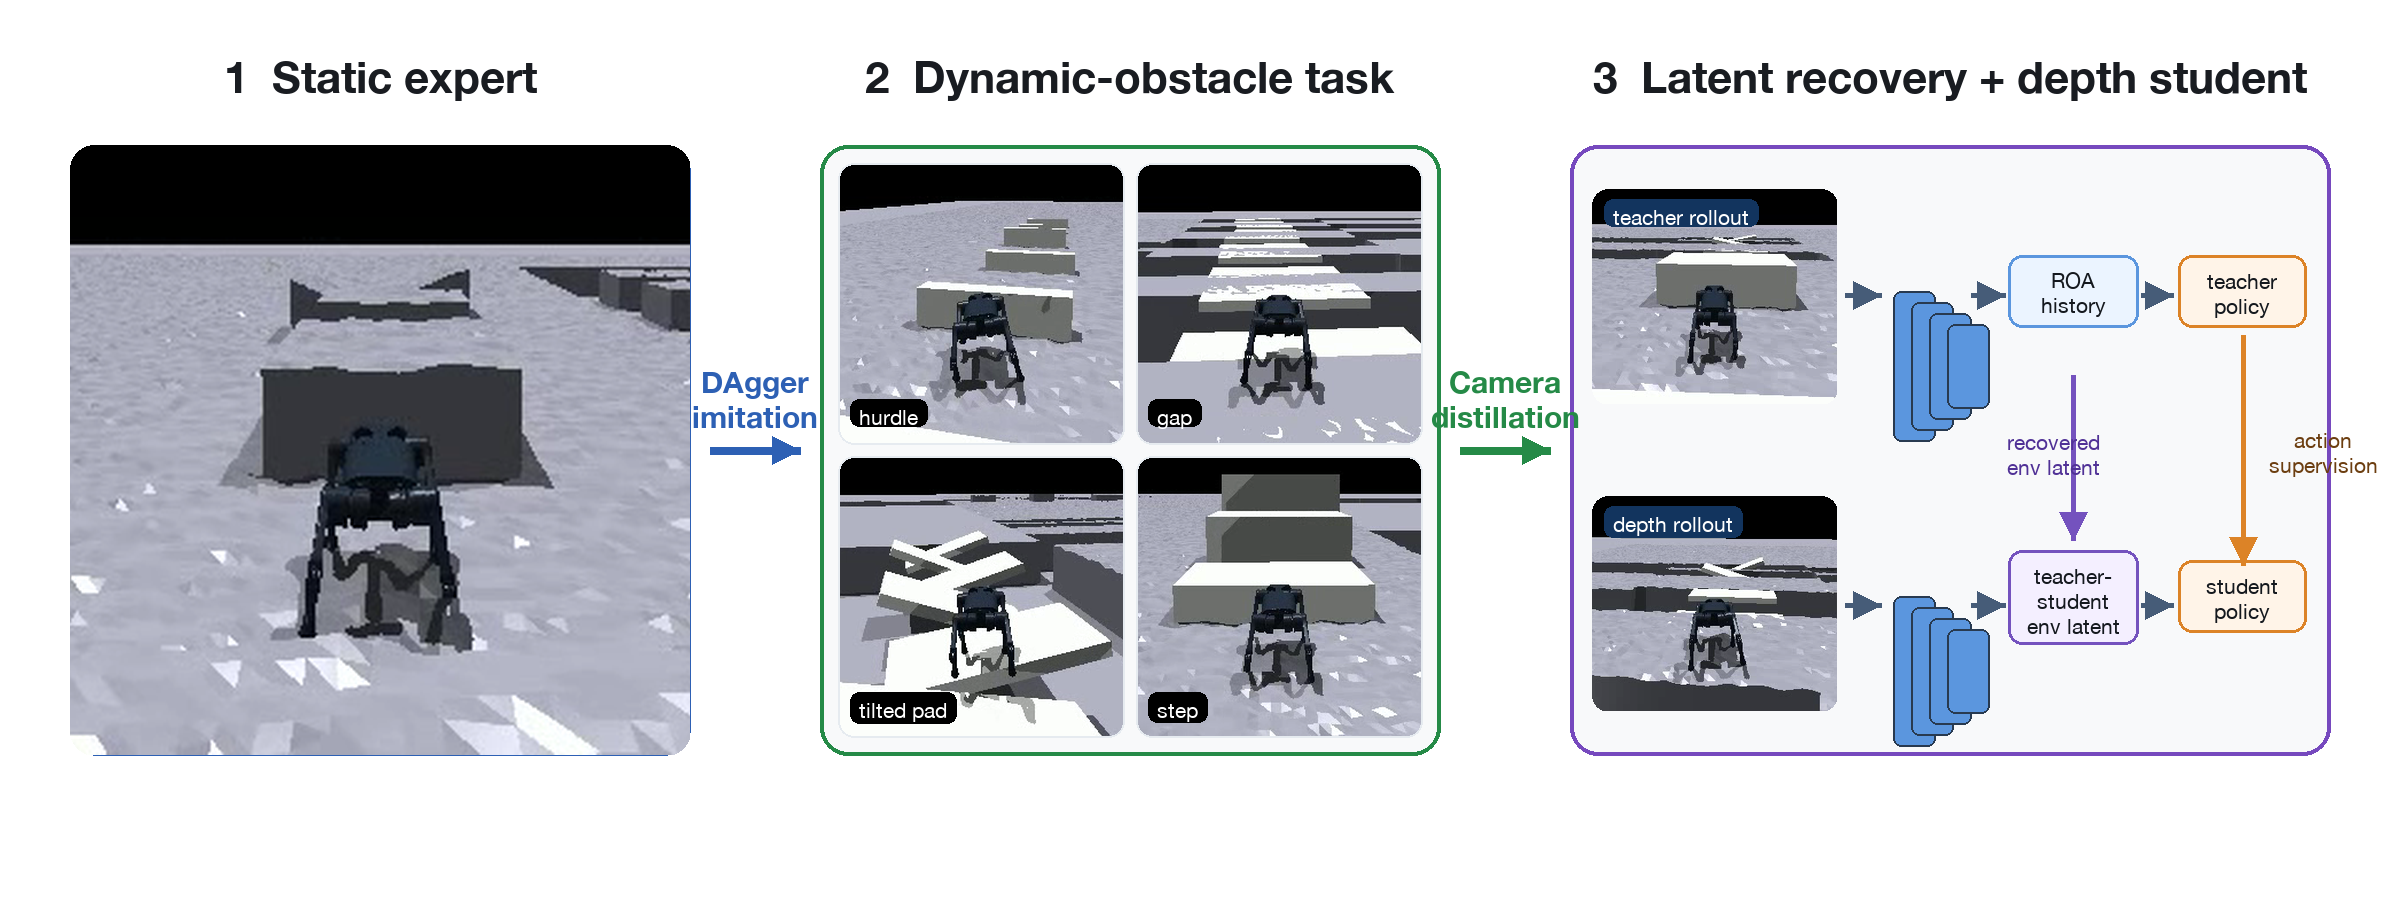
\includegraphics[width=0.98\textwidth]{training_pipeline_ai.png}
	\vspace{-2.5em}
	\caption{Training pipeline overview. A static parkour expert provides imitation targets for dynamic-terrain pretraining, the privileged dynamic policy is fine-tuned with obstacle-state latents, and the deployable depth student uses hybrid recovery to keep useful dynamic obstacle state while suppressing harmful latent labels.}
	\label{fig:pipeline}
\end{figure*}

\subsection{Baseline Static Parkour Pipeline}
The baseline task uses a curriculum grid of terrain tiles. Rows control difficulty, columns select terrain families, and each tile contains eight navigation goals. The policy is rewarded for progress toward the current goal and heading alignment, while penalties discourage collisions, unstable posture, torque spikes, and foot placement near terrain edges. Height scans provide privileged exteroception during base training, and depth images replace this scan information during camera distillation.

% \begin{figure}[htbp]
% 	\centering
% 	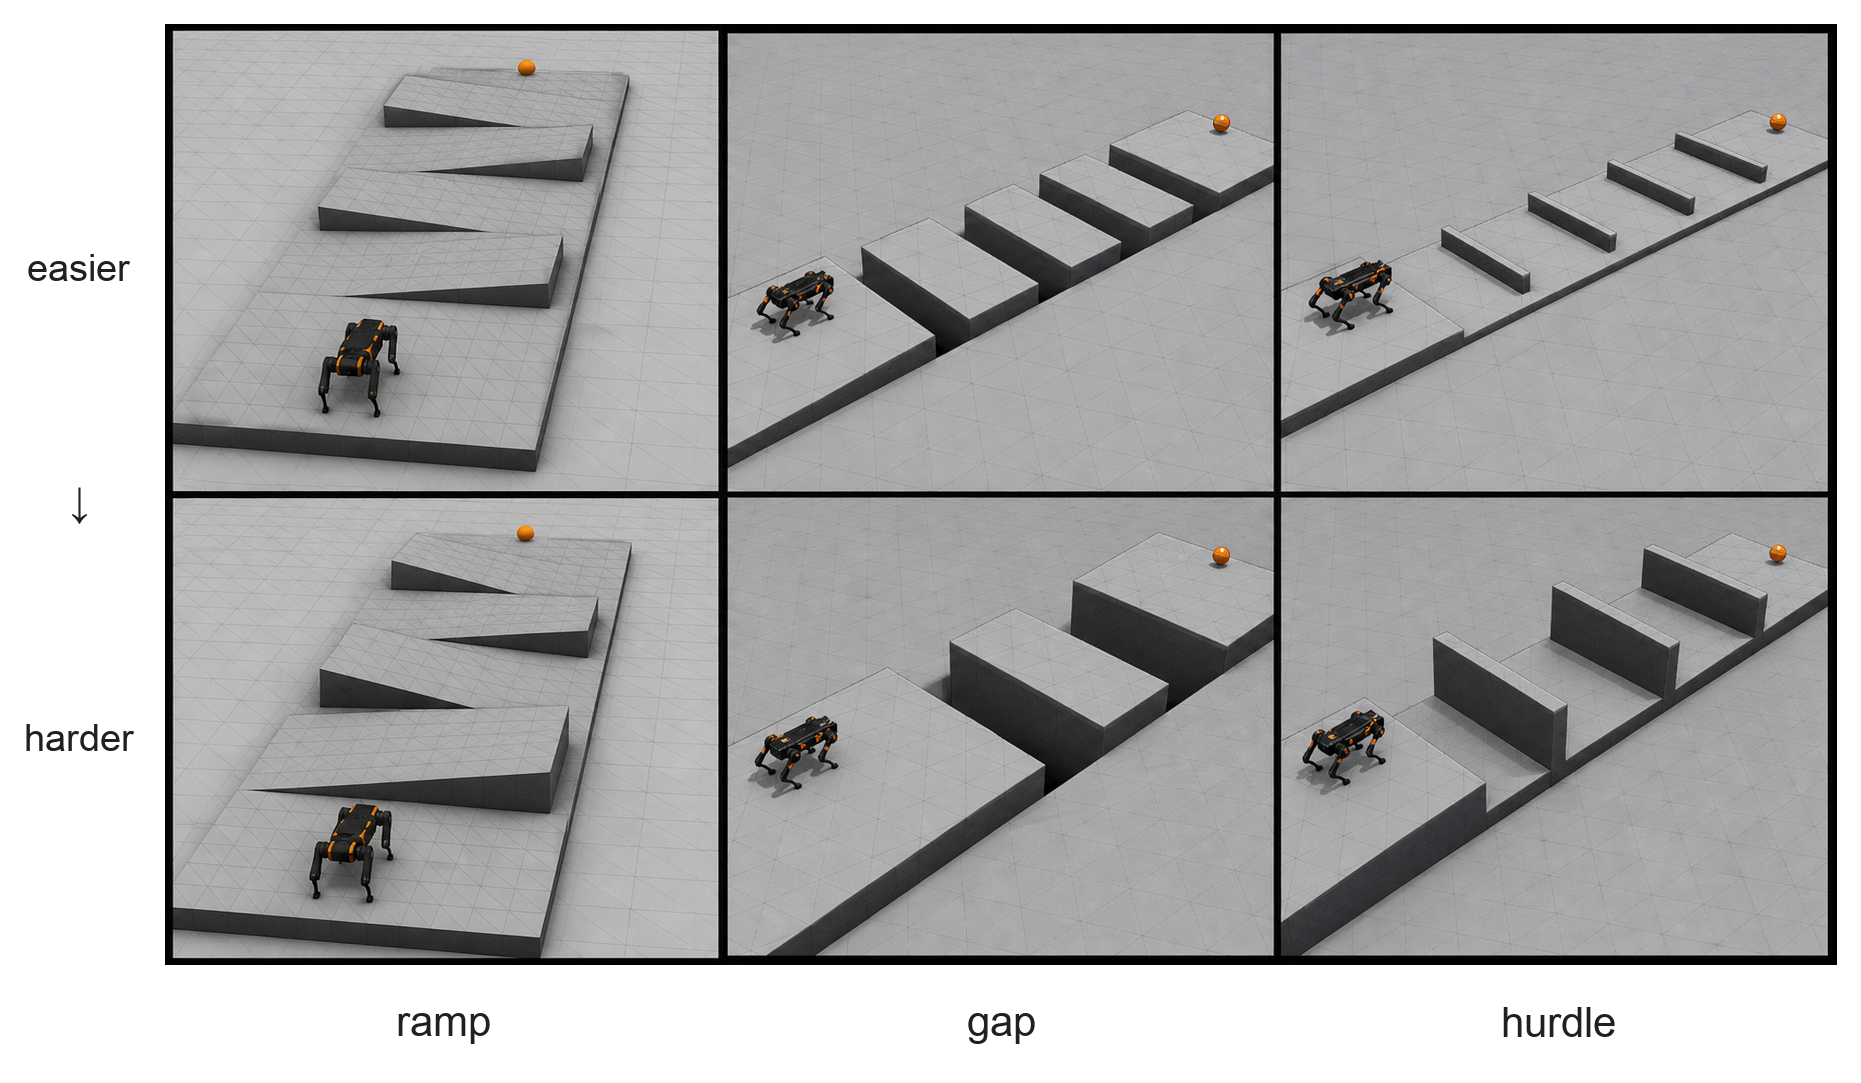
\includegraphics[width=\linewidth]{curriculum_tiles_labeled.png}
% 	\caption{Curriculum structure: columns select obstacle families, while rows control difficulty.}
% 	\label{fig:curriculum}
% \end{figure}

The baseline training stack has two latent recovery paths. First, during base reinforcement learning, a history encoder learns to match privileged latent variables from recent proprioceptive observations. Second, during camera distillation, a depth encoder predicts scan-derived latent information and yaw correction so that the deployment policy can act without privileged terrain scans. Dynamic parkour stresses both mechanisms because obstacle state may be visible before contact, only inferable after contact, or not useful at all.

\subsection{Dynamic-Obstacle Task Infrastructure}
The \texttt{a1\_dynamic} task keeps the A1 robot, eight-goal course interface, curriculum shape, and observation contract of the original task, but replaces static terrain families with dynamic obstacle families. It is registered as a separate task and uses a dynamic-specific environment class so that the original \texttt{a1} task remains available.

Dynamic terrain generation separates static foundations from moving obstacle metadata. The heightfield still provides the ground mesh and coarse course layout. In addition, each tile stores the dynamic family, difficulty, obstacle dimensions, motion type, motion group, goal-to-motion mapping, and per-slot actor specifications. Each environment has six obstacle groups and two actor slots per group. Hurdles, tilted pads, and steps use one active slot and one inactive parked slot; gaps use both slots for moving takeoff and landing supports.

At runtime, dynamic obstacles are gravity-disabled Isaac Gym box actors. The environment creates these actors after the robot actor, resets their poses when a robot is assigned to a new curriculum tile, and updates their root states before physics steps. Hurdles translate along the forward axis, gap platforms translate as paired supports, tilted pads rotate about roll, and steps move vertically.

Obstacle motion is scripted by sinusoidal signals. For each obstacle group, the curriculum difficulty interpolates obstacle-type-specific motion parameter ranges before the environment uniformly samples the actual amplitude and period. Random phase offsets decorrelate obstacle timing across environments. Gap tiles synchronize phase across all gap groups so that takeoff and landing supports move consistently and stably.

On top of the original static height scan, the dynamic environment additionally overlays the current top surfaces of active obstacle actors. Goals tied to moving supports, namely gap takeoff and landing platforms, are translated with the same motion groups so the policy targets the current traversable surface.

The dynamic task exposes a unified configuration interface for the main obstacle families. Hurdles vary in height, thickness, translation amplitude, and period. Gaps vary in gap width, platform dimensions, translation amplitude, and period. Tilted pads vary in lateral placement, roll amplitude, and period. Steps vary in mean height range, vertical amplitude, and period. Curriculum difficulty interpolates these ranges before uniform sampling.

\subsection{DAgger-Style Imitation Pretraining}
Training dynamic parkour from scratch is difficult because early failures prevent the policy from reaching informative states. We therefore add an imitation pretraining stage before dynamic base reinforcement learning. The expert is a static-terrain A1 policy.

\begin{algorithm}[htb]
	\small
	\caption{DAgger-style imitation pretraining}
	\label{alg:dagger}
	\begin{algorithmic}[1]
		\Require static expert \(\pi_E\), dynamic environment
		\State Initialize student \(\pi_\theta\)
		\State Initialize teacher replay buffer \(B_E\) and student replay buffer \(B_S\)
		\For{\(k=0,\dots,K-1\)}
		\If{\(k\) is the BC warmup iteration}
		\State Roll out \(\pi_E\) and store \((o,\pi_E(o))\) in \(B_E\)
		\Else
		\State Roll out \(\pi_E\) and append labeled states to \(B_E\)
		\State Roll out \(\pi_\theta\) and label visited states with \(\pi_E\)
		\State Append student-induced samples to \(B_S\)
		\EndIf
		\State Sample a balanced minibatch from \(B_E\) and \(B_S\)
		\State Update \(\pi_\theta\) with action, history-action, and estimator losses
		\EndFor
		\State \Return \(\pi_\theta\) for base RL fine-tuning
	\end{algorithmic}
\end{algorithm}

The imitation objective trains both the privileged actor path and the history-encoding actor path. It also trains the estimator used by the original pipeline, so the resulting checkpoint can be consumed by the normal base-RL runner. When dynamic environment latent augmentation is enabled, imitation also supervises the masked dynamic-state recovery losses for families assigned to ROA-style recovery.

\subsection{Dynamic Environment Latent Augmentation}
We augment the environment latent with a low-dimensional dynamic obstacle state appended after the original privileged latent slice. For \texttt{a1\_dynamic}, this vector has 30 dimensions: two upcoming obstacle groups, each represented by 15 features. Static \texttt{a1} keeps this dimension at zero.

Each group contains validity and type bits, relative geometry, motion state, and motion parameters. Table~\ref{tab:dynamic_latent_features} summarizes the per-group feature layout.
\begin{table*}[htb]
	\caption{Per-group dynamic latent features.}
	\label{tab:dynamic_latent_features}
	\centering
	\begin{tabular}{lll}
		\toprule
		Category & Variable & Meaning \\
		\midrule
		Validity & \(\mathbf 1_{\mathrm{valid}}\) & whether this upcoming obstacle group is valid \\
		Type bits & \(\mathbf 1_{\mathrm{hurdle}}, \mathbf 1_{\mathrm{gap}}, \mathbf 1_{\mathrm{step}}, \mathbf 1_{\mathrm{pad}}\) & one-hot indicators for hurdle, gap, step, and tilted pad \\
		Relative geometry & \(x_0, x_1\) & robot-relative forward positions of slot 0 and slot 1 \\
		& \(y\) & robot-relative lateral offset of the obstacle group \\
		Primary state & \(v_{\mathrm{primary}}, \dot{v}_{\mathrm{primary}}, \ddot{v}_{\mathrm{primary}}\) & family-specific scalar state and its time derivatives \\
		Motion phase & \(\sin\varphi, \cos\varphi\) & current phase of the scripted motion \\
		Motion parameters & \(A, \omega\) & sampled amplitude and angular frequency \\
		\bottomrule
	\end{tabular}
\end{table*}
The primary value \(v_{\mathrm{primary}}\) is family-specific: hurdle top height, effective gap width, step top height, or tilted-pad roll angle. The representation is intentionally redundant: a compact low-dimensional signal may otherwise be too weak to affect policy decisions, but extra state can distract from robust behavior when it is not useful.

Recovery mode is configured per obstacle family. In ROA-style recovery, the history encoder predicts obstacle state during base RL and the policy later consumes the recovered history latent. In teacher-student recovery, the depth encoder predicts obstacle state during camera distillation. A hybrid configuration can assign different obstacle families to different recovery paths.

\subsection{Mixed Terrain and Latent Suppression}
The per-family ablations showed that not all dynamic obstacle state should be exposed. Gap state is strongly tied to visual timing: the robot benefits from knowing where the moving takeoff and landing supports are. Tilted-pad state was a negative improvement in both ROA-style and teacher-student experiments. Hurdle state was also not consistently helpful; the dominant difficulty appeared to be robustness to contact and collision artifacts rather than precise phase recovery.

The final \texttt{a1\_\allowbreak mixed} task keeps the dynamic infrastructure but changes the terrain mixture and latent mask. It uses \texttt{mixed\_\allowbreak hurdle}, \texttt{dynamic\_\allowbreak gap}, \texttt{mixed\_\allowbreak tilted\_\allowbreak pads}, \texttt{parkour\_\allowbreak step}, and \texttt{mixed\_\allowbreak demo}. The \texttt{mixed\_\allowbreak hurdle} and \texttt{mixed\_\allowbreak tilted\_\allowbreak pads} courses retain the same visible moving actors as their dynamic counterparts, but suppress obstacle state features. The gap family keeps dynamic latent recovery. \texttt{dynamic\_\allowbreak step} is replaced by the static \texttt{parkour\_\allowbreak step} because the current dynamic step actor generated poor learning signals and frequent collision-induced failures.

\subsection{Depth Encoder Scan-Latent Loss}
We add an optional scan-latent matching loss during camera distillation:
\[\mathcal L_{\mathrm{scan}}=\left\|z_{\mathrm{scan}}-z_{\mathrm{depth}}\right\|_2.\]
When enabled, it is added to the existing depth actor update:
\[\mathcal L=\mathcal L_{\mathrm{action}}+\mathcal L_{\mathrm{yaw}}+w_{\mathrm{dynamic}}\mathcal L_{\mathrm{dynamic}}+\mathcal L_{\mathrm{scan}}.\]
The loss was intended to stabilize the depth latent that replaces privileged scan information. As shown in the experiments, it did not produce a substantial improvement in mean waypoints.

\section{Experiments}
\subsection{Setup and Metrics}
We compare the baseline pipeline on static terrain, the baseline pipeline applied directly to dynamic terrain, imitation-pretrained dynamic training, environment latent augmentation (ELA) with different recovery modes, ELA with hybrid recovery mode (HELA) on mixed terrain, and HELA with depth encoder loss.

The primary metric is mean waypoints, defined as the proportion of waypoints (goals) reached during evaluation. It measures progress through the eight-goal course and is more interpretable than reward alone for parkour. We also report mean reward as it helps identify cases where a run collects auxiliary reward (e.g., heading alignment, upright posture, and collision avoidance) without making comparable parkour progress.

\subsection{Original Pipeline Degradation}
Figure~\ref{fig:baseline_curves} shows that the original pipeline does not transfer directly from static to dynamic terrain. The static base run reaches nearly 1.0 waypoint, while the dynamic base run remains far lower even after longer training. Camera distillation preserves the same gap: static distillation remains strong, and dynamic distillation remains weak.

\begin{figure*}[htbp]
	\centering
	\includegraphics[width=0.48\textwidth]{static_dynamic_waypoints.pdf}
	\hfill
	\includegraphics[width=0.48\textwidth]{distillation_waypoints.pdf}
	\caption{Baseline pipeline degradation from static to dynamic terrain. Left: base-RL training curves. Right: camera distillation curves, with dashed lines showing base-RL references.}
	\label{fig:baseline_curves}
\end{figure*}

Common failure modes are family-specific. Hurdles destabilize the body when they move during contact. Gaps require takeoff and landing to be timed against moving support surfaces. For dynamic steps, the robot receives little reward and does not learn the emergent behavior of placing the front legs on the step.

\subsection{Imitation Pretraining}
DAgger-style pretraining improved dynamic learning by placing the policy near a useful static-parkour behavior before dynamic training. The fine-tuned base policy after imitation pretraining reached much higher mean waypoints than the dynamic baseline.

% \begin{figure}[htbp]
% 	\centering
% 	\includegraphics[width=\linewidth]{imitation_losses.pdf}
% 	\caption{Imitation pretraining losses. The student learns privileged action imitation, history-branch action imitation, and estimator targets before dynamic base-RL fine-tuning.}
% 	\label{fig:imitation_losses}
% \end{figure}

\subsection{ELA, Latent Recovery, and HELA}

Environment latent recovery was evaluated by obstacle family. Figure~\ref{fig:recovery_modes} compares no-ELA, pure ROA-style recovery, pure teacher-student recovery, and the resulting HELA configuration. These per-family ablations determine the HELA design: gap uses teacher-student recovery, hurdle and tilted-pad variants suppress dynamic latent labels, and dynamic step is replaced by the static \texttt{parkour\_\allowbreak step}.

\begin{figure*}[htbp]
	\centering
	\includegraphics[width=0.80\textwidth]{recovery_mode_training_curves.pdf}
	\caption{Per-family waypoint curves for recovery modes. The upper row shows base RL and the lower row shows camera distillation; dashed lines in the distillation row mark corresponding base-RL references.}
	\label{fig:recovery_modes}
\end{figure*}

\subsection{Depth Encoder Loss}
The depth encoder scan-latent loss was tested on top of HELA. Figure~\ref{fig:depth_loss} compares camera distillation with and without this loss. The added supervision does not clearly improve mean waypoints over the same HELA run without the extra loss.

\begin{figure}[htbp]
	\centering
	\includegraphics[width=\linewidth]{depth_loss_distill_comparison.pdf}
	\caption{HELA camera distillation with and without the depth encoder scan-latent loss. The dashed line marks the shared base-RL reference.}
	\label{fig:depth_loss}
\end{figure}

\section{Results and Discussion}
\subsection{Deployment Performance Comparison}
Table~\ref{tab:pipeline_comparison} summarizes the deployment-stage performance of all pipelines. The baseline static policy reaches \(0.936\) mean waypoints. Applying the original pipeline directly to dynamic terrain drops to \(0.230\). Our improved HELA pipeline recovers to \(0.808\), substantially reducing the gap to static-terrain performance. Adding the depth encoder loss reaches \(0.748\), which is not a meaningful improvement over HELA.

\begin{table}[htb]
	\centering
	\caption{Deployment-stage comparison of all pipelines.}
	\label{tab:pipeline_comparison}
	\begin{tabular}{llcc}
		\toprule
		Pipeline & Terrain & Waypoints & Reward \\
		\midrule
		Baseline & Static & \textbf{0.936} & 18.26 \\
		Baseline & Dynamic & \textbf{0.230} & 8.85 \\
		Imitation only & Dynamic & 0.538 & 17.93 \\
		ELA + ROA & Dynamic & 0.497 & 15.50 \\
		ELA + teacher-student & Dynamic & 0.510 & 16.64 \\
		HELA & Mixed & \textbf{0.808} & 16.69 \\
		HELA w/ depth enc. loss & Mixed & 0.748 & 16.06 \\
		\bottomrule
	\end{tabular}
\end{table}

\subsection{Family-Specific Latent Recovery}
The per-family recovery-mode ablation results in Figure~\ref{fig:recovery_modes} explain the HELA design. Gap traversal benefits most from teacher-student recovery because takeoff and landing timing estimation requires visual information about moving support surfaces. Hurdle performance is strongest without ELA: hurdle motion is small, and collision artifacts dominate the failure mode. Tilted-pad augmentation hurts because the robot can aim for the rotation axis, making roll angle less useful and turning explicit obstacle state into a training distraction. Dynamic step is currently unusable because step-actor collisions push the robot back strongly and prevent reward collection. HELA therefore routes gap state through teacher-student recovery, suppresses hurdle and tilted-pad dynamic labels, and replaces dynamic step with static \texttt{parkour\_\allowbreak step}.

\subsection{Imitation Pretraining}
As shown in Table~\ref{tab:pipeline_comparison}, imitation pretraining alone already brings substantial improvement over the baseline pipeline. This indicates that initialization matters in dynamic parkour. The task is sparse and contact-rich; without a reasonable behavior prior, the policy often fails before it reaches informative obstacle interactions. DAgger-style pretraining from a static expert gives a useful starting distribution for later reinforcement learning and latent recovery.

\subsection{Depth Encoder Loss}
As shown in Figure~\ref{fig:depth_loss}, adding depth encoder loss did not bring improvements over HELA. Direct scan-latent matching is intuitively appealing because it gives the depth pathway an additional supervised target, but action imitation and dynamic-state supervision already provide strong gradients for the representation needed by HELA. In other words, the policy does not necessarily need an exact reconstruction of the teacher's internal scan representation to obtain sufficient environmental information for parkour. Therefore, the added loss may over-constrain the intermediate representation.

\section{Conclusion}
This project extends static A1 parkour to dynamic-obstacle parkour and evaluates how the original privileged-to-depth pipeline can be adapted. The implemented dynamic task provides moving obstacle actors, dynamic height scans, moving goals, and a configurable family-level interface. Our proposed training pipeline, HELA, combines DAgger-style static-expert pretraining, dynamic environment latent augmentation, family-specific latent recovery, mixed-terrain latent suppression, and an optional depth encoder loss.

Experimental results show that the original pipeline degrades severely on dynamic terrain, while HELA recovers most of the lost performance. The best-performing system uses a family-specific latent recovery mode: gap state is recovered visually, while hurdle and tilted-pad state are suppressed. Adding depth encoder loss did not bring improvement over HELA, suggesting that direct scan-latent matching can make the learned representation too constrained. Future work should add timing metrics such as takeoff error and landing stability and stress-test depth recovery under degraded sensing conditions such as latency, jitter, and frame drops.

\bibliographystyle{plainnat}
\bibliography{references}

\appendices
\section{Author Contributions}
Zhijie Chen led the system design, algorithm implementation, experiment design and execution, data analysis, and paper writing. His contributions include dynamic-obstacle infrastructure, DAgger-style imitation pretraining, environment latent augmentation with different recovery modes, hybrid latent recovery and mixed terrain design, depth encoder loss integration, task tuning, ablation experiments, the proposal, the midterm report, oral presentation slides, and the paper.

Shiyi Xiao explored possible dynamic-obstacle parkour task solutions during the project.

\end{document}
